\section{Mathematical Model}
\label{ch:mathmodel}

As per the base and periodic models shown in \cite{grigor20}.

\subsection{Base model}

\begin{figure}[!htb]
\minipage{0.48\textwidth}
  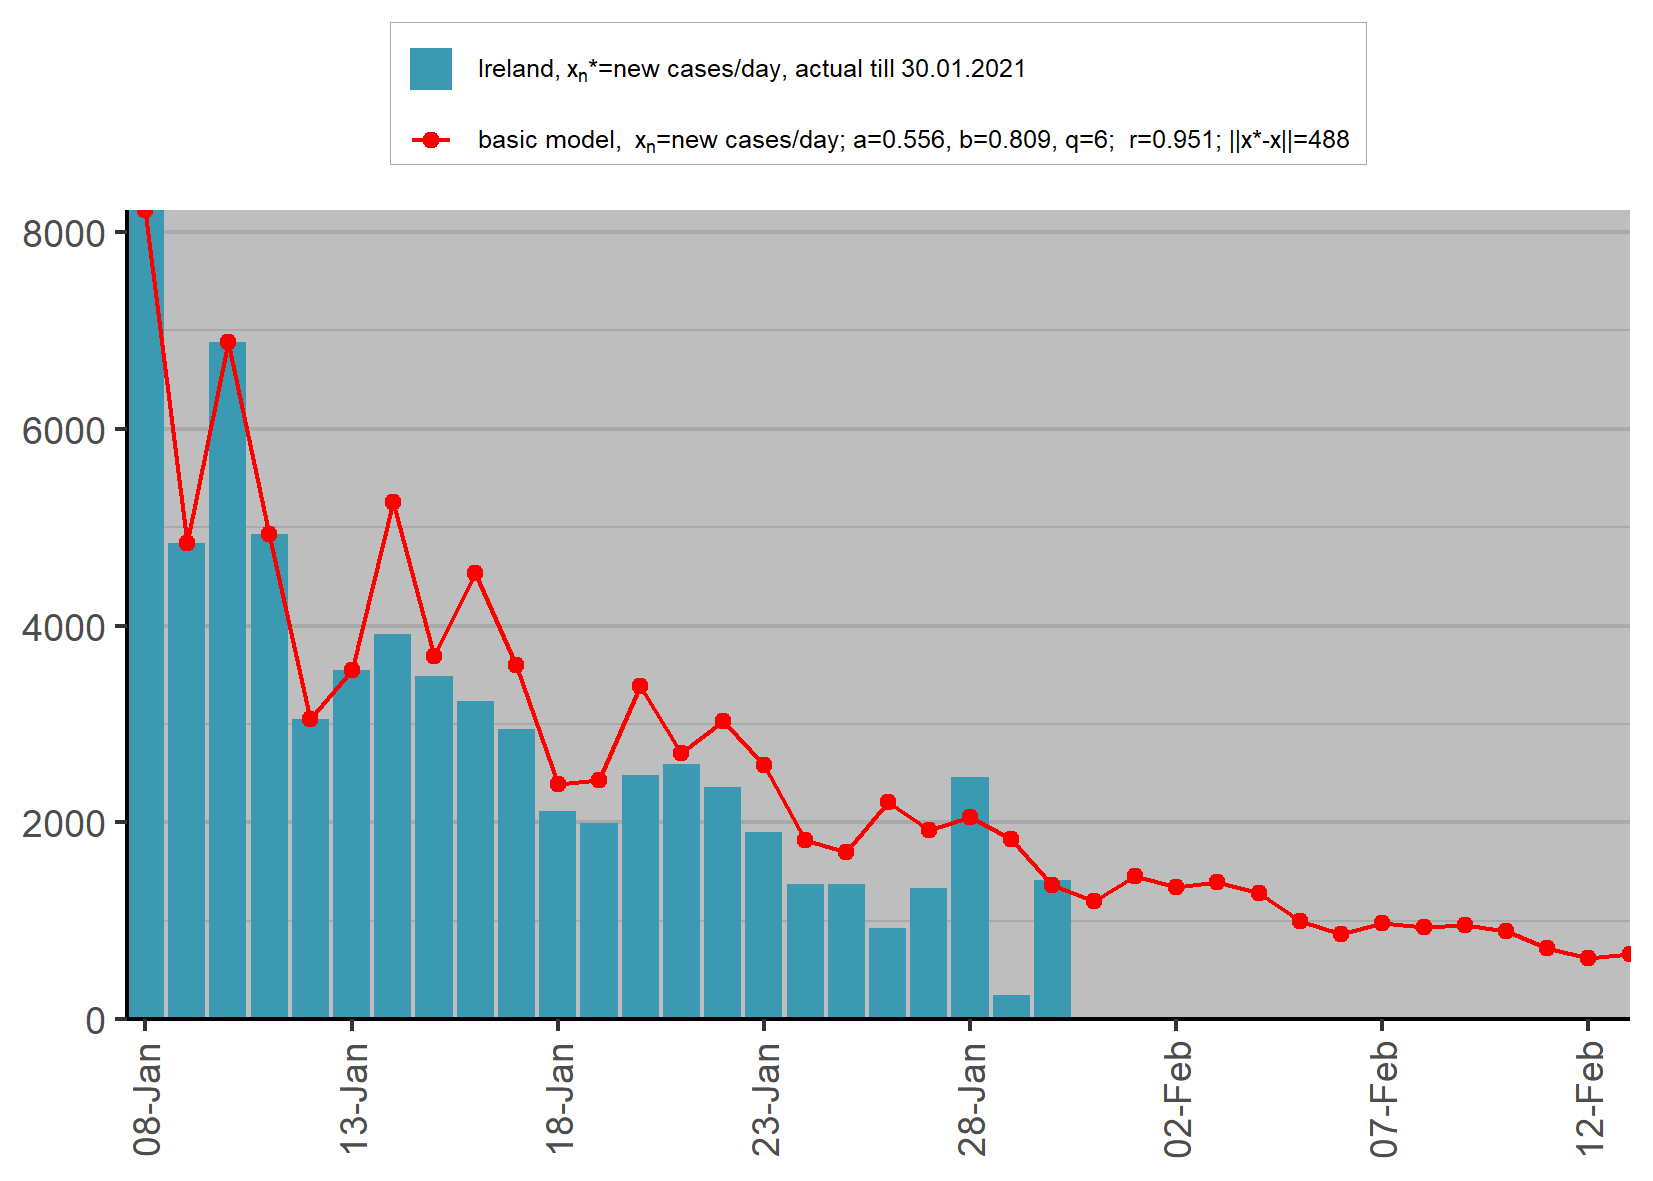
\includegraphics[width=\linewidth]{Ireland-basexn.png} \label{fig:ireland-basexn}
\endminipage\hfill
\minipage{0.48\textwidth}
  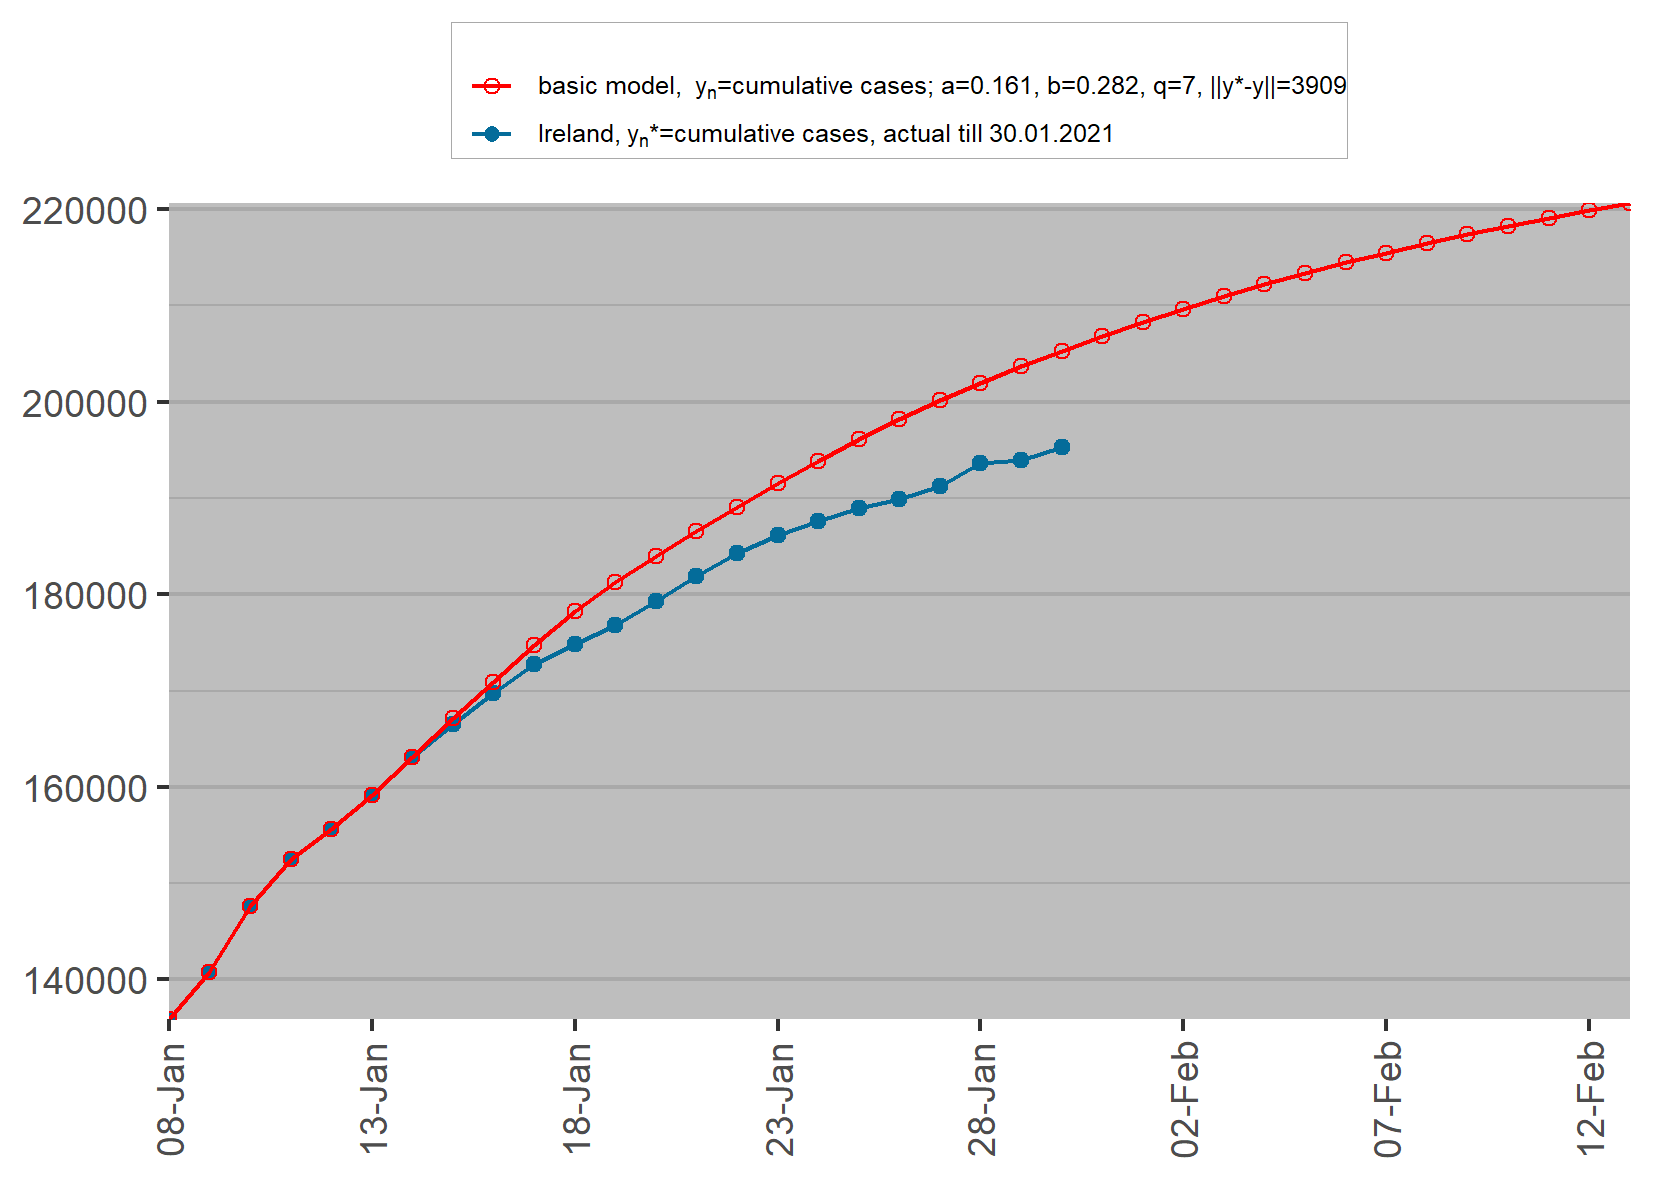
\includegraphics[width=\linewidth]{Ireland-baseyn.png} \label{fig:ireland-baseyn}
\endminipage
\caption{Basic modelsl, Ireland}
\end{figure}

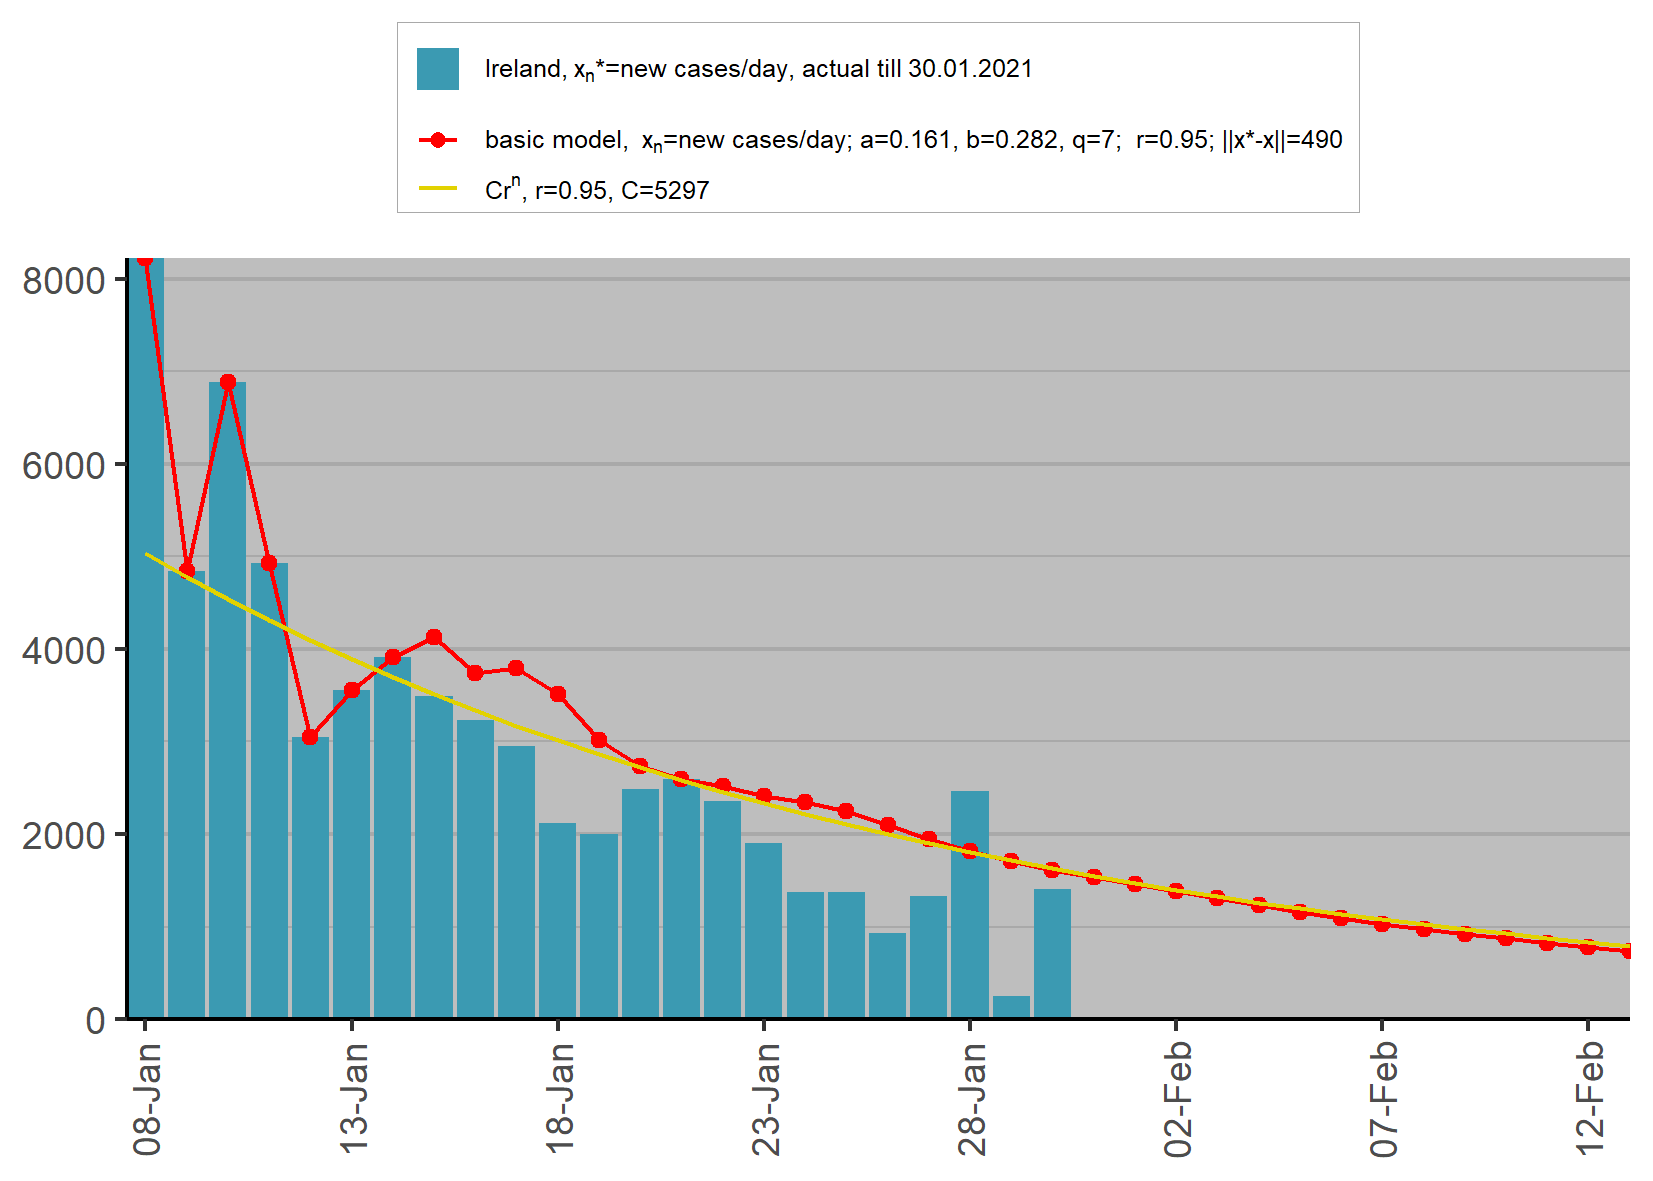
\includegraphics[width=0.9\textwidth]{Ireland-Crn.png}

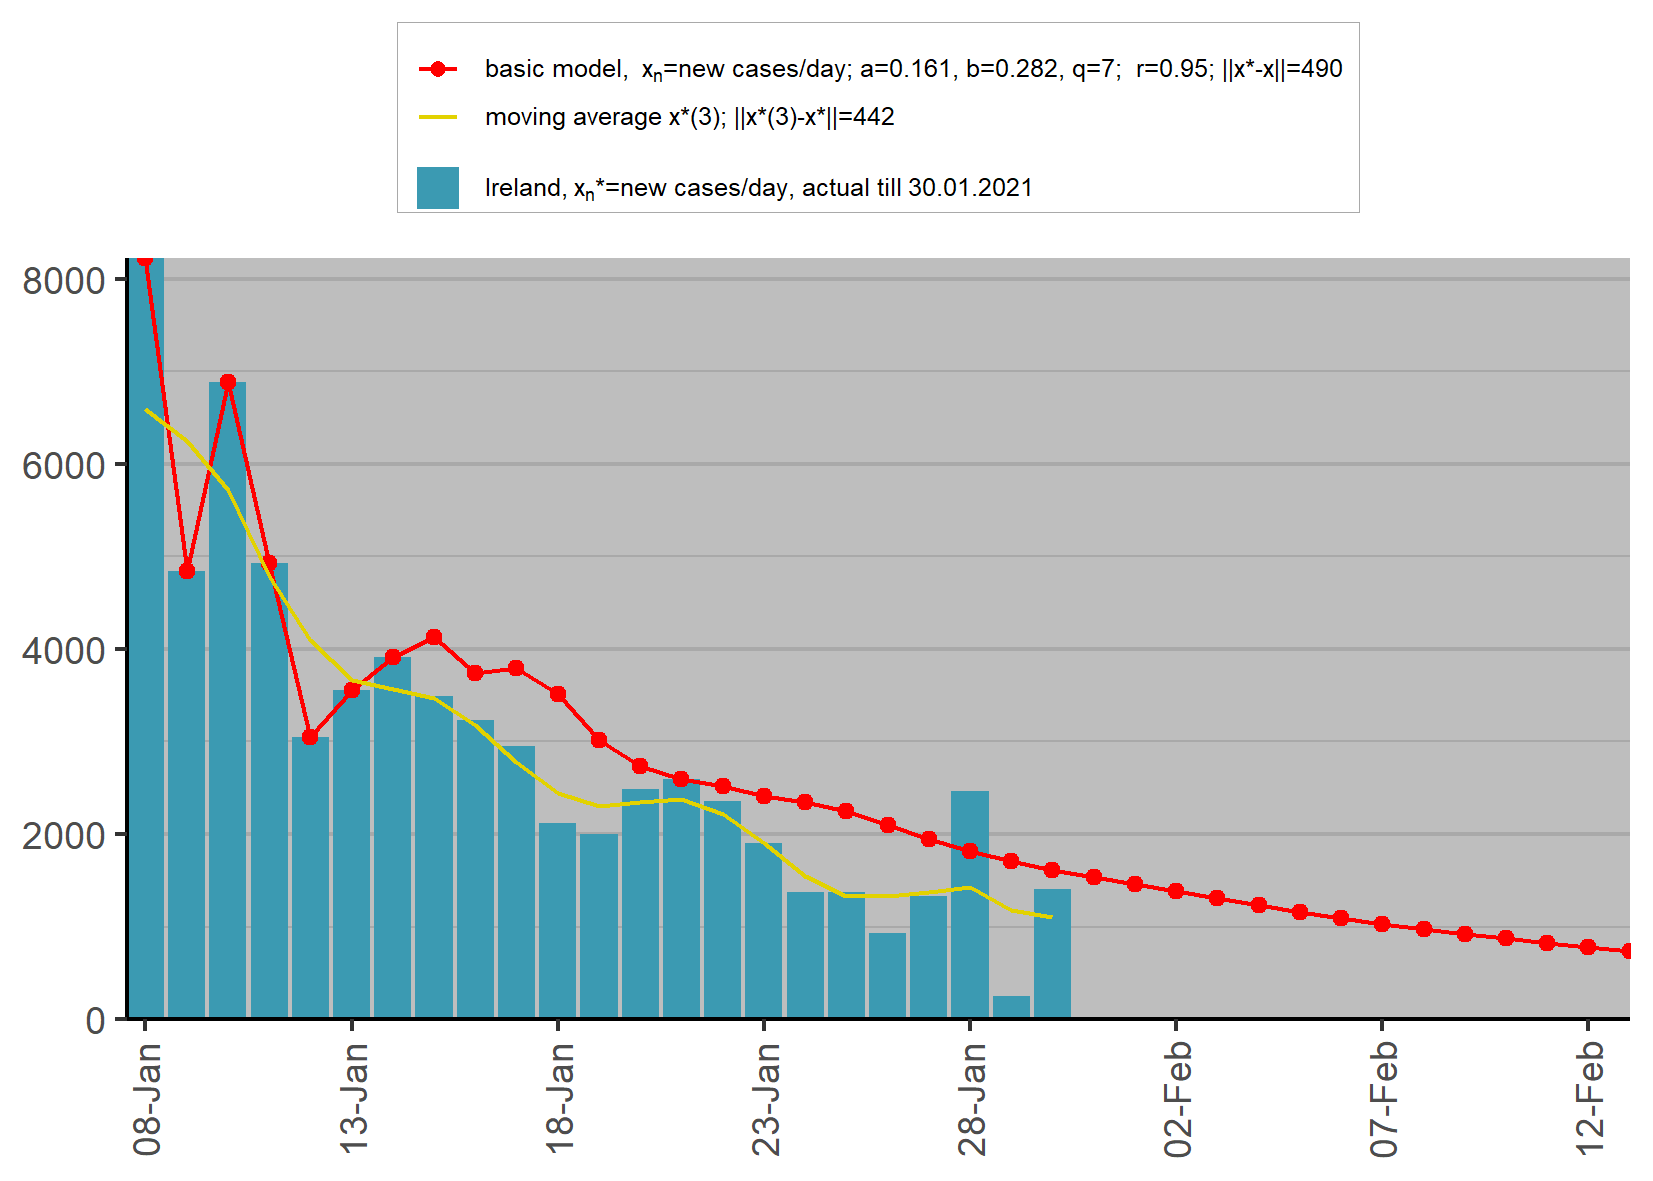
\includegraphics[width=0.9\textwidth]{Ireland-mavgx3.png}


\subsection{Periodic model}

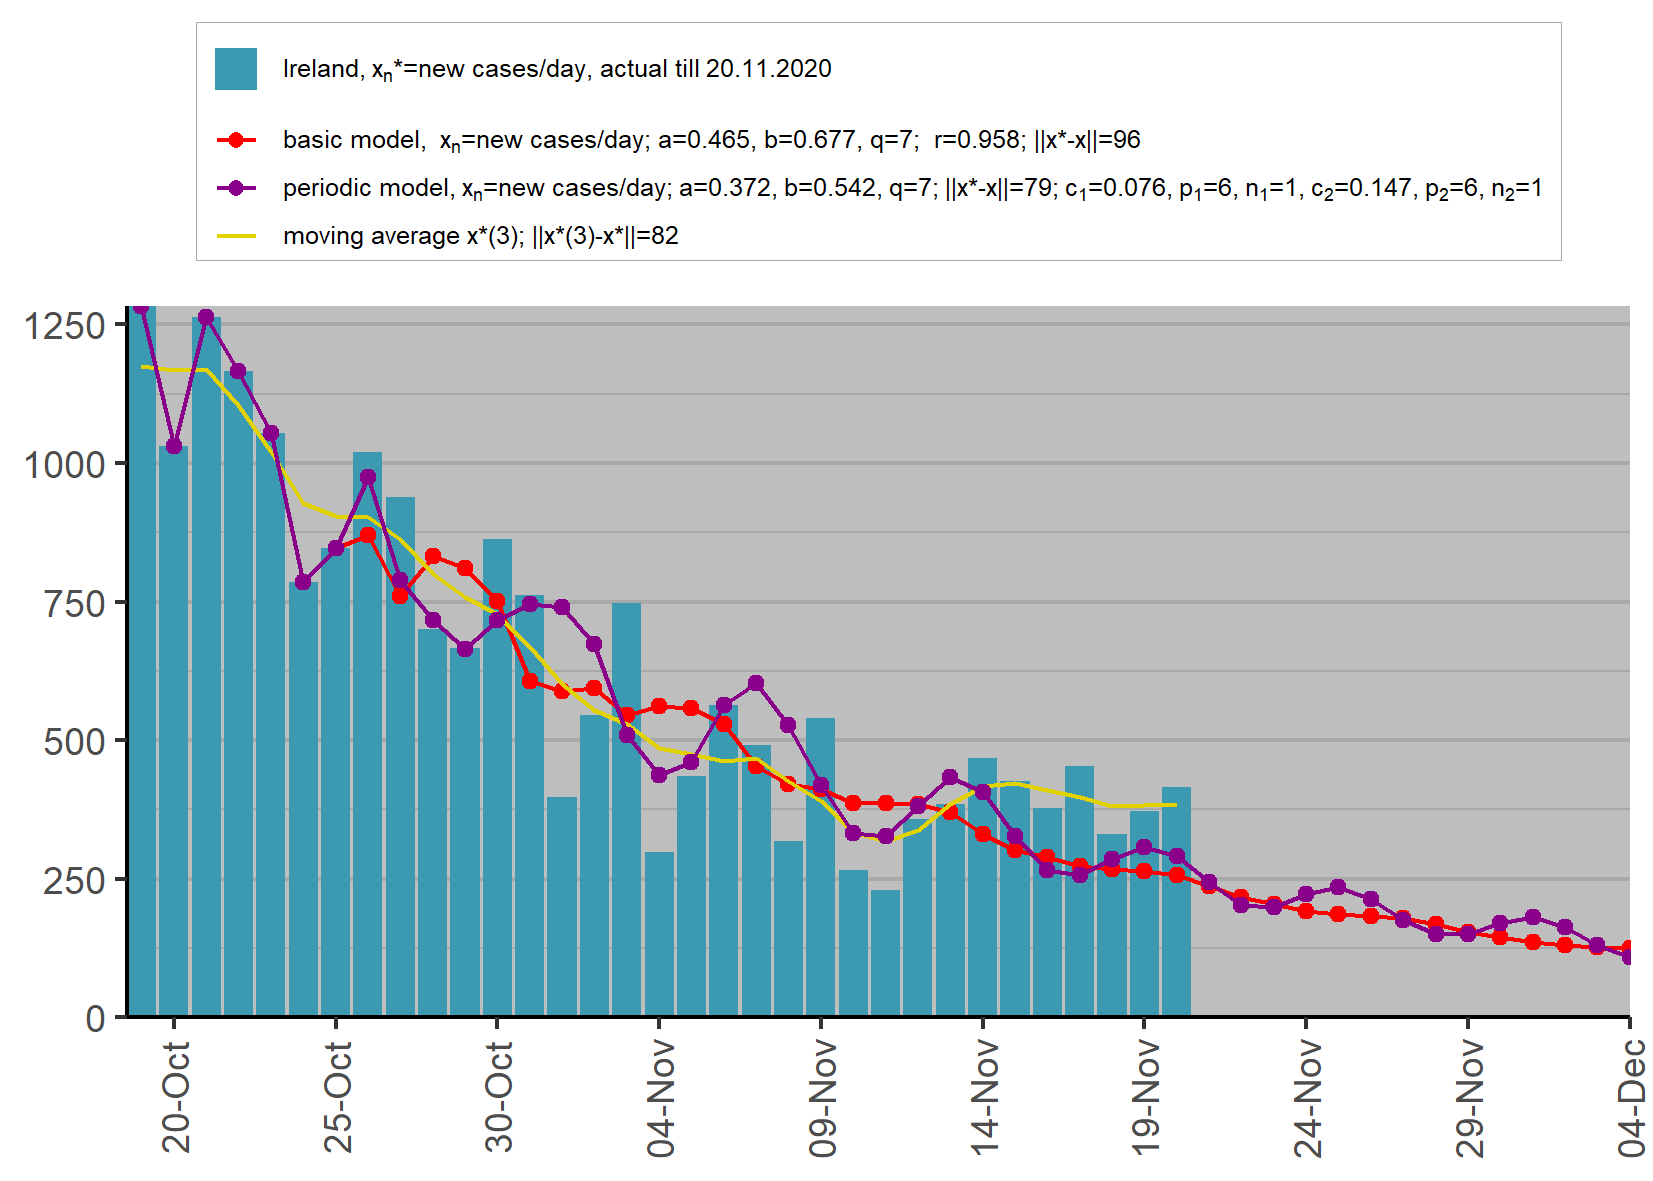
\includegraphics[width=0.9\textwidth]{Ireland-periodic.png}


\subsection{Multi-phase model}

\begin{figure}[!htb]
\minipage{0.48\textwidth}
  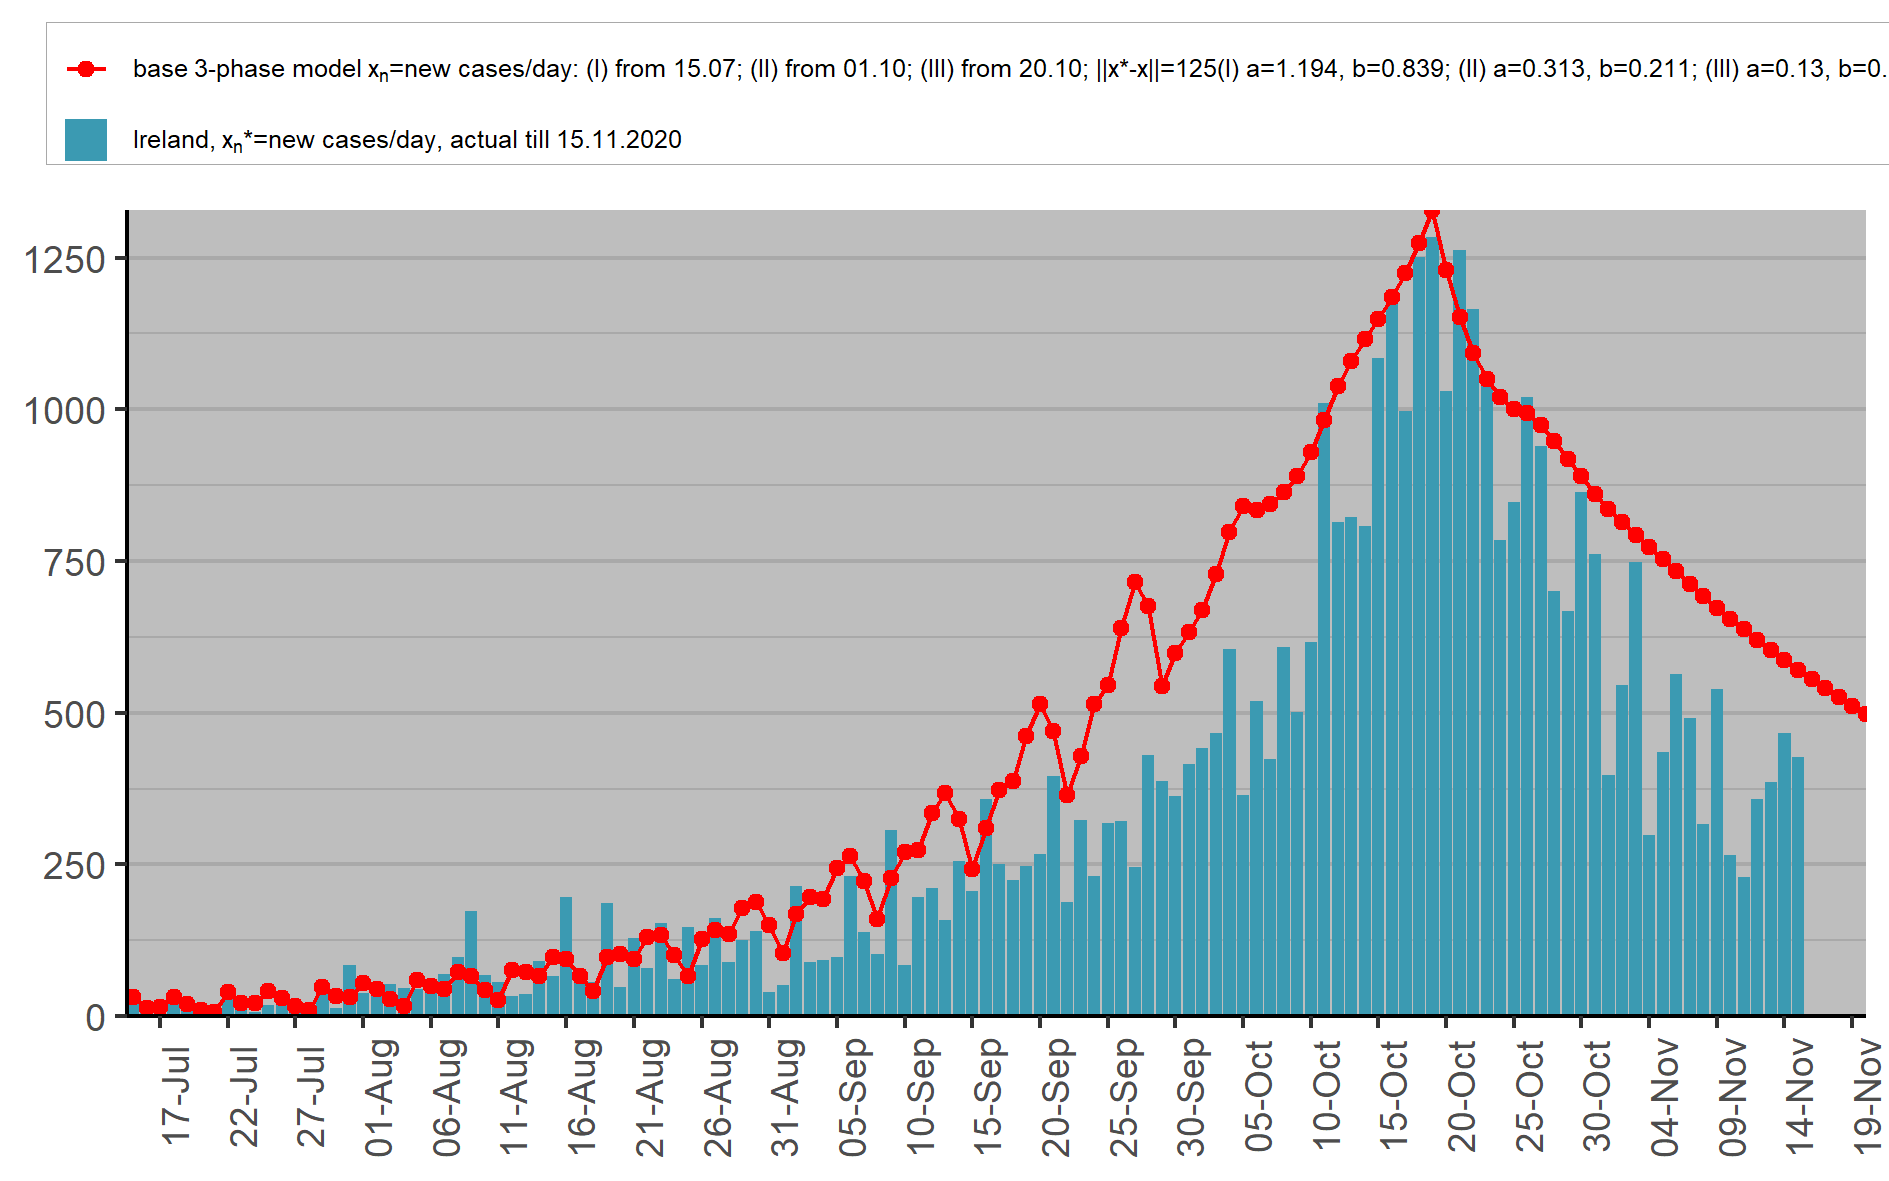
\includegraphics[width=\linewidth]{Ireland-xnmult.png} \label{fig:ireland-xnmult}
\endminipage\hfill
\minipage{0.48\textwidth}
  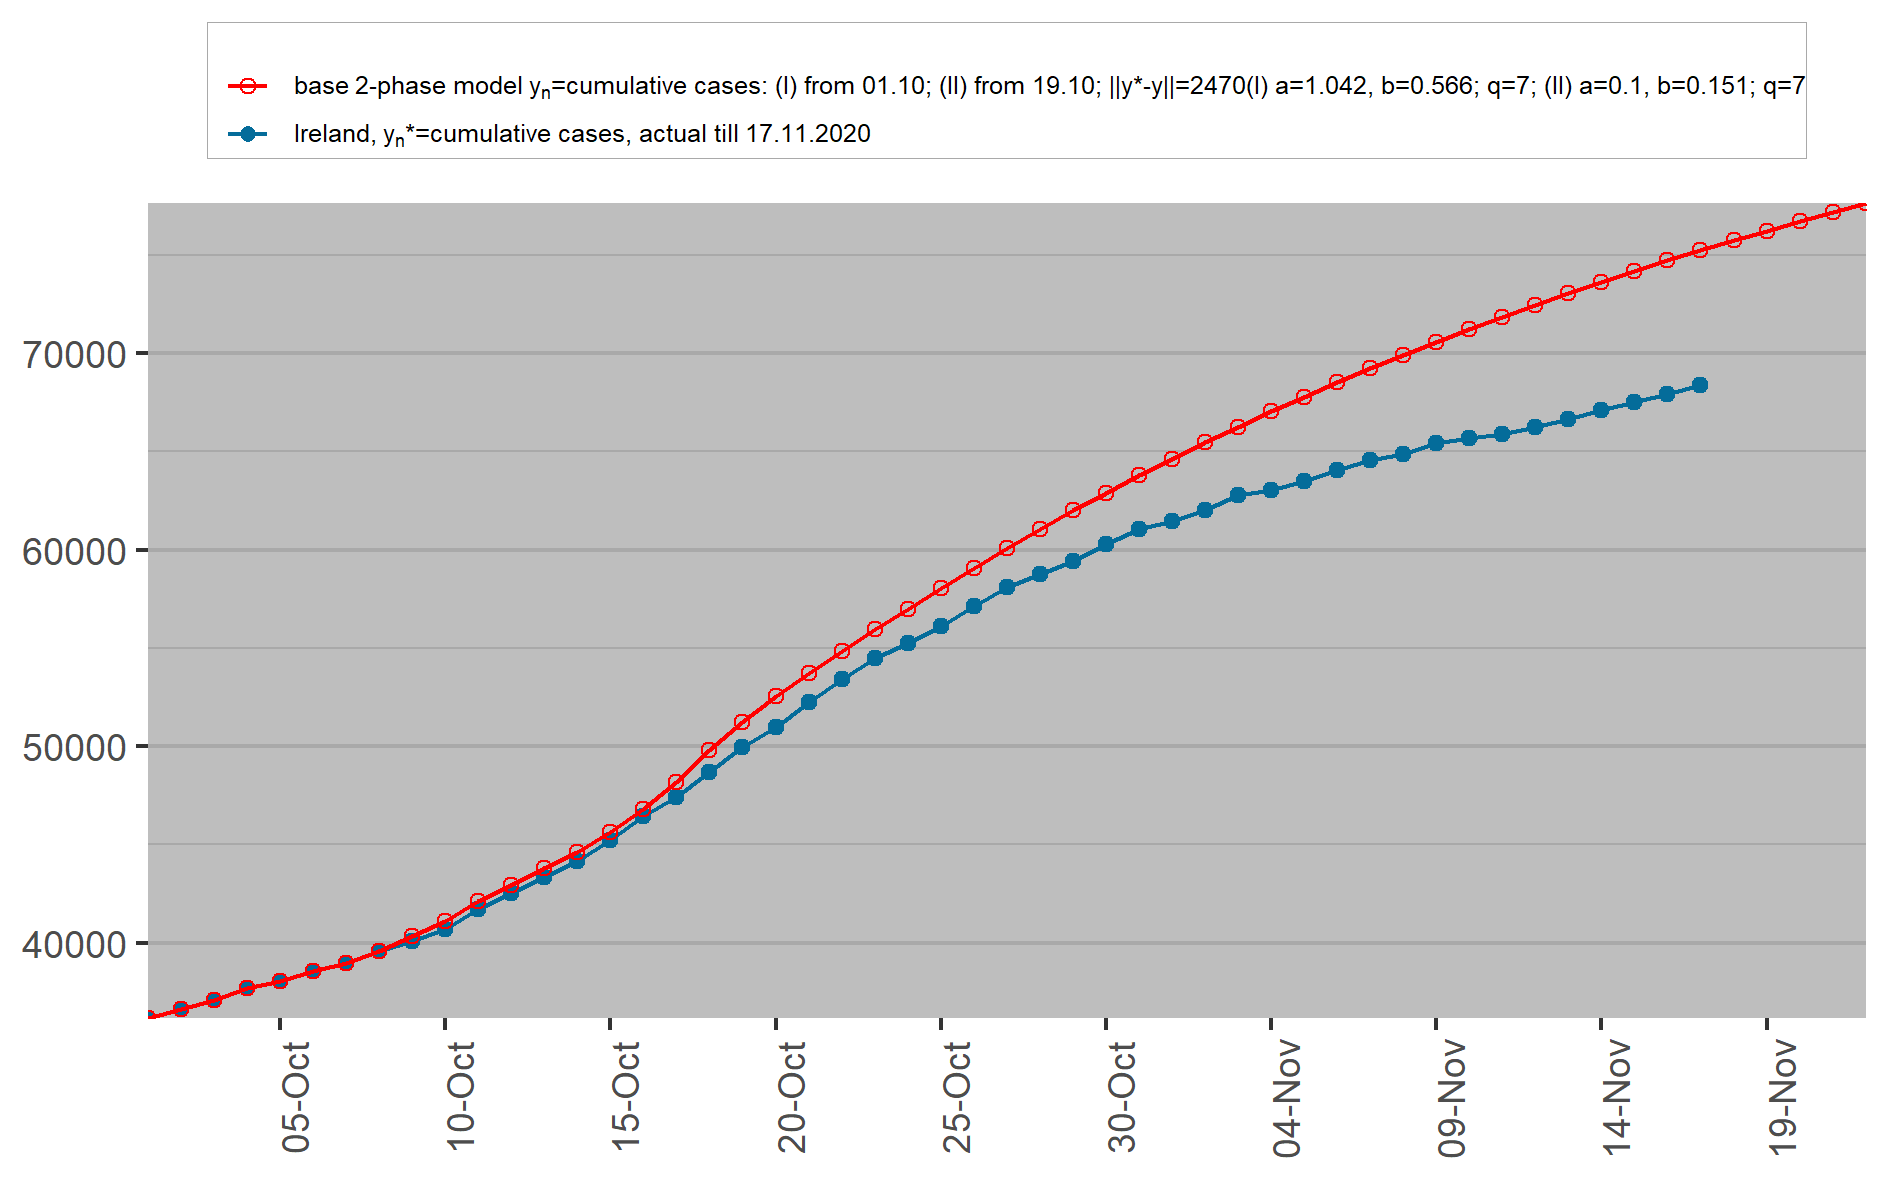
\includegraphics[width=\linewidth]{Ireland-ynmult.png} \label{fig:ireland-ynmult}
\endminipage
\caption{Multi-phase model, Ireland}
\end{figure}

\begin{figure}[!htb]
\minipage{0.48\textwidth}
  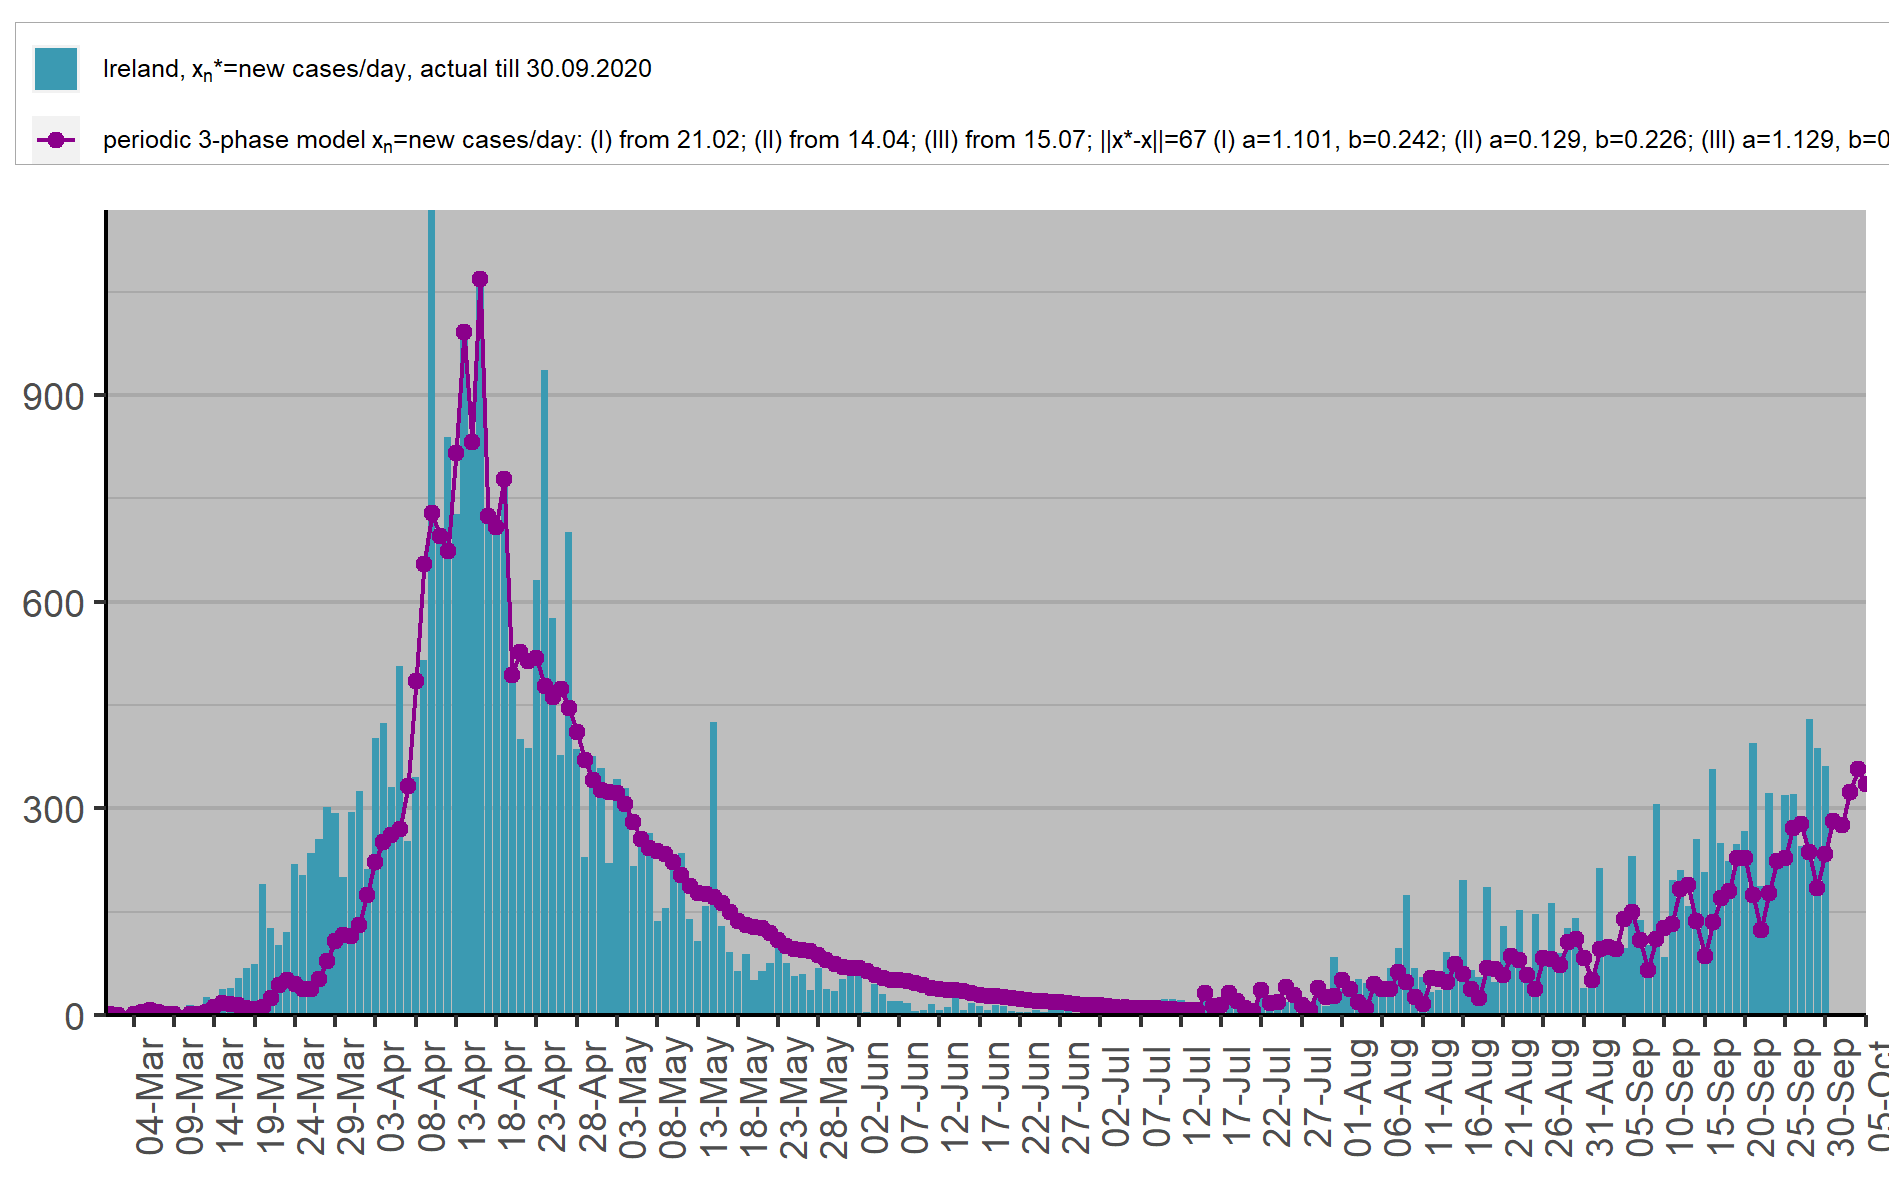
\includegraphics[width=\linewidth]{Ireland-perxnmult.png} \label{fig:ireland-perxnmult}
\endminipage\hfill
\minipage{0.48\textwidth}
  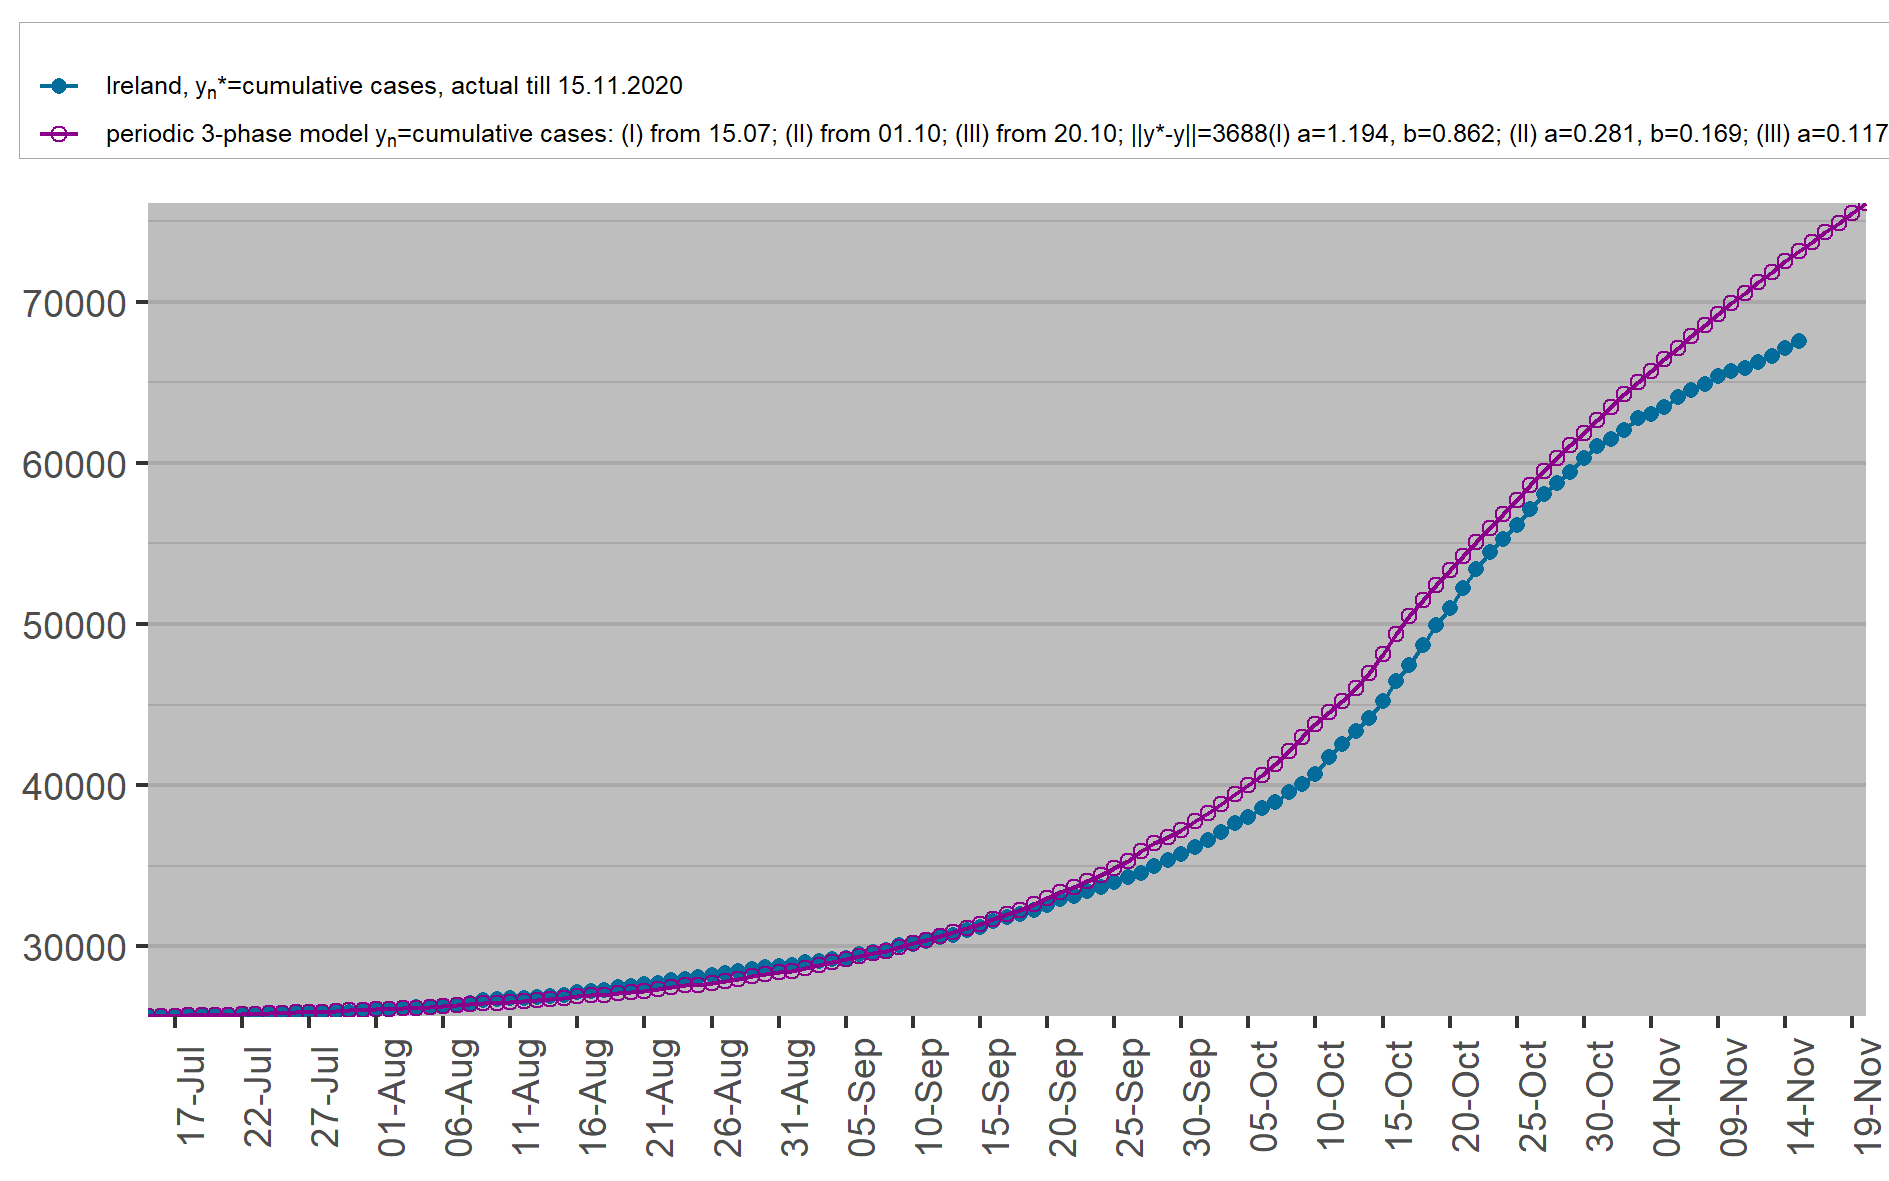
\includegraphics[width=\linewidth]{Ireland-perynmult.png} \label{fig:ireland-perynmult}
\endminipage
\caption{Multi-phase periodic model, Ireland}
\end{figure}

